%\ihead{\headmark}
\chapter{Deep Learning}

Deep learning is a subfield of machine learning which in fact, is a subfield of Artificial Intelligence (AI). Deep learning has emerged as one of the most exciting field of computer science, and it is keep expanding its scope. It has been used in many technologies such as, in medical to identify the diseases, automatic game playing, self-driving cars, image recognition, natural language processing and many more. The reason why deep learning is successful in many different domain is its ability to understand multiple levels of representation of data. Its mean that, it not only has ability to classify and predict, but also has ability to learn different level of complexity. Before diving into deep learning, it is necessary to understand a broader field "machine learning".

\section{Machine Learning}

Machine Learning [1] is a data analysis method. It gives the computer the ability to learn from data without being explicitly instructed. By using different machine learning algorithms, it helps to find hidden insights of data and allow us to build models to make predictions. It can be classified into 2 categories.

\begin{enumerate}
	\item Supervised Learning
	\item Unsupervised Learning
\end{enumerate}

\subsection{Supervised Learning}

In supervised learning, the labeled data is used to train the models. Here, labeled data represents that we know the input and output variables in advance. Thus, we know what we are looking for and then we use an algorithm to come up with a mapping function which maps the input variables to the output variables. Learning is supposed to be stopped when the level of performance reaches to the desired result. Supervised learning is generally divided into regression and classification.
\begin{itemize}
	\item \textbf{Regression}: A problem in which the output variable is a category.
	\item \textbf{Classification}: A problem in which the output variable is the real value.
\end{itemize}

\subsection{Unsupervised Learning}

In unsupervised learning, we only have input data and no corresponding output variables. Thus, there are no labels given and it is expected to find the structure in the data itself, i.e. finding hidden patterns to learn more about data. It is different from supervised learning in that we don't know what will be the correct value. Unsupervised learning is generally divided into clustering and association.

\begin{itemize}
	\item \textbf{Clustering}: Group objects in such a way that the objects, which are similar to each other, placed in the same cluster.
	\item \textbf{Association}: Discover rules that define the large portions of the data such as people who buys product X may buy Y as well.
\end{itemize}

The objective of machine learning is to analyze the past and present data and predict or make a decision for the future data. In supervised learning, the basic work flow is to build a model, evaluate or tune a model and then deploy it in the production environment where it will do the predictions. The work flow can be seen in figure.


\begin{figure}[htpb]
	\centering
	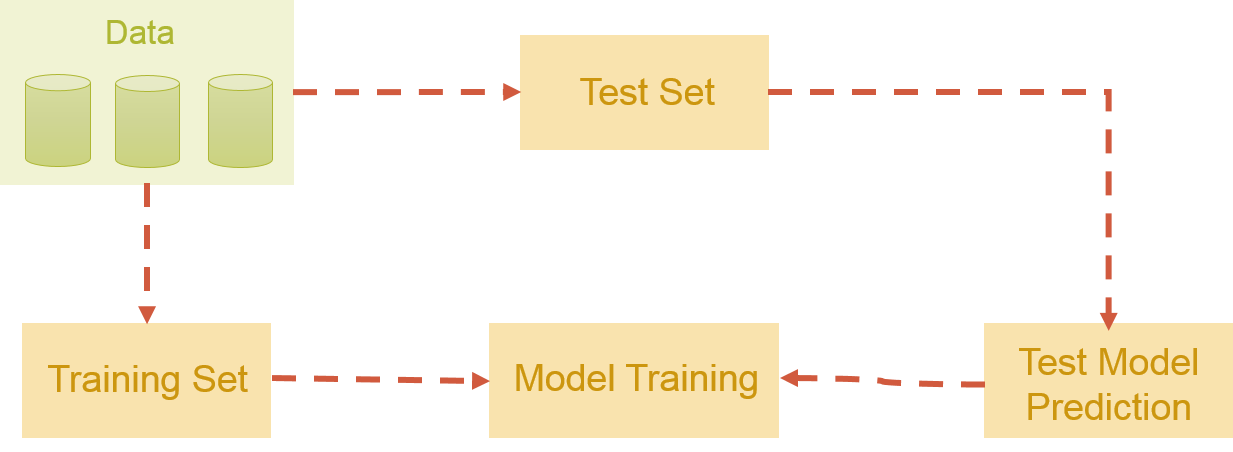
\includegraphics[width=12cm,height=10cm,keepaspectratio=true]{images/basic-ml-model.png}
	\caption{
		Basic supervised machine learning workflow.
	}
	\label{fig:basic-ml-model}
\end{figure}


Machine learning is generally powered by a huge amount of data which is generally referred aa Big Data. It is generally defined as a too big or complex data which cannot be processed on a single machine. As the data is growing day by day, the new tools are also required to process that big data on multiple machines and extract the useful insights from the data.


One of the problem with the traditional machine learning model is the feature extraction challenge. The model designer or the programmer needs to specifically tells the model which features it should consider to make a correct decision. The model heavily relies on the programmer's understanding of data and this was a huge burden on the programmers. For a problems like object recognition, language translation, it was a huge problem.

Deep learning comes into play to solve the problem of feature extraction. They have the capability to focus only on the right features by themselves by understanding as much data as possible, requiring very little input from the programmer. This feature of deep learning models makes it very powerful tool for the current machine learning era.




\section{Artificial Neural Networks}
Artificial neural networks (ANNs) are generally inspired by the biological neural networks that mimics brain functionality \cite{wiki:ann}. These systems generally learned by considering examples instead of specifically define rules for certain situations or cases. An ANN is a network of nodes called artificial neurons which are connected to other neurons using a link called synapse. Each neuron gets the input, process the input and pass the output to the next neuron.
In most basic state, an ANN consists of 3 layers:

\begin{enumerate}
	\item Input Layer
	\item Hidden Layer
	\item Output Layer
\end{enumerate}

\begin{figure}[htpb]
	\centering
	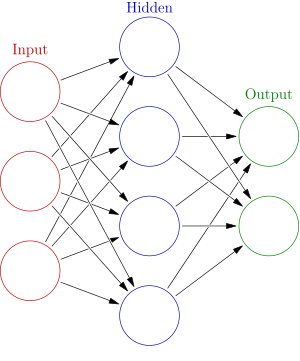
\includegraphics[width=6cm,height=10cm,keepaspectratio=true]{images/neural-net}
	\caption{
		An artificial neural network with its 3 basic layers, taken from \cite{wiki:ann}.
	}
	\label{fig:wiki:ann}
\end{figure}


\subsection{Artificial Neuron}
An artificial neuron is the most basic unit of ANN. It consist of inputs and produces an output. Generally, the inputs are multiplied by some weights to specify which inputs are more important. The higher the value of weights, the more important they are. The inputs are shown as a, b and c and weights as $w_1$, $w_2$ and $w_3$ in figure \ref{fig:single-neuron}. After then the products are summed together and passed to the activation function. An activation function is a function which takes an input an generates an output based on certain threshold. So, if the summed value is greater than the threshold value of that activation function, the output is produced or in other terms, the neuron fired else no output is produced and neuron does not fired.

\begin{figure}[htpb]
	\centering
	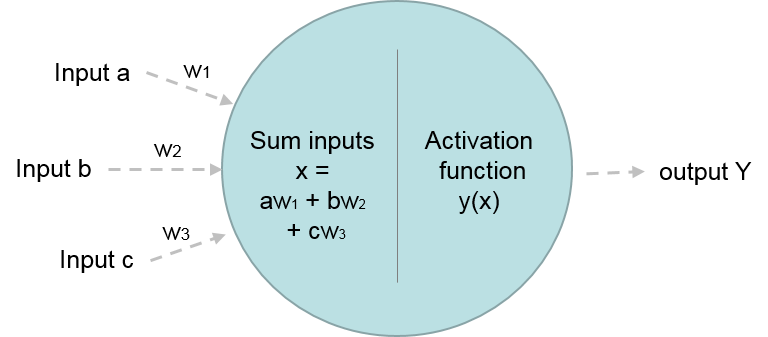
\includegraphics[width=10cm,height=10cm,keepaspectratio=true]{images/single-neuron}
	\caption{
		A single artificial neuron.
	}
	\label{fig:single-neuron}
\end{figure}

Artificial neurons adjust the weights as the learning proceeds and the process of finding weights is known as learning. ANN considers many different examples and find the best possible combination of weights to provide the most accurate results. There are many other parameters involved as well to find a good combination of weights.

\subsection{Activation Function}

A function that takes an input and produce output based on threshold value is known as activation function \cite{ujjwalkarn}. There are many step functions available. Few of them are:

\subsubsection{Sigmoid}
It takes a real value input and scale it to the range of 0 to 1. It is also known as logistic function. It is represented as:

\begin{center}
$y = \frac{1}{1 + e^{-x}}$
\end{center}

The another variation of sigmoid function is softmax function which is used for multiclass classification.

\subsubsection{Tanh}
It takes a real value input and scale it to the range of -1 to 1. It is also a sigmoidal function as it also takes s-shaped.


\subsubsection{ReLU}
It stands for Rectified Linear Unit. It is the most used activation function as it is the ideal choice to be used in convolutional neural networks. It takes the real value input and all negative values are mapped to zero. It is represented as:

\begin{center}
$f(x) = max(0, x)$
\end{center}

\begin{figure}[htpb]
	\centering
	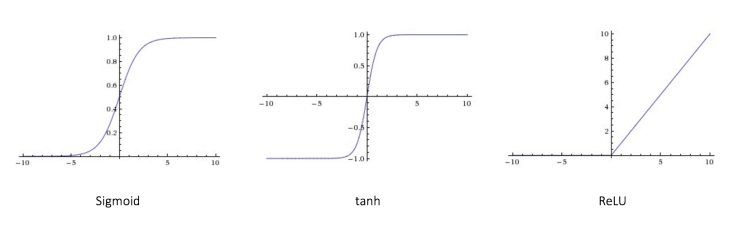
\includegraphics[width=15cm,height=10cm,keepaspectratio=true]{images/act-funcs}
	\caption{
		Activation functions, taken from \cite{ujjwalkarn}.
	}
	\label{fig:funcs}
\end{figure}

The graph of all the activation functions defined above can be seen in figure \ref{fig:funcs}.

\subsection{Convolutional Neural Network}